% Appendix Template
\setstretch{1.3}
\chapter{Additional Temporal Tweezers} % Main appendix title
\label{AppendixC} % Change X to a consecutive letter; for referencing thI_{\sigma} appendix elsewhere, use \ref{AppendixX}
\lhead{Appendix D. \emph{Additional Temporal Tweezers}}
\setstretch{2}

In this Appendix, we present additional tweezing results for the full LL Eq.~(\ref{eq:LLETweeze}) with the same analysis presented in Sec.~\ref{section:TweezeResults}.  Figure~\ref{fig:ACSkinnyQ} depicts the density of the power ratios (a) inside $Q_{\rm I}$ and (b) outside $Q_{\rm O}$ of a tweezer with width $\sigma_\phi = 0.5$ and $h_\phi = 2$.  For the full LL Eq.~(\ref{eq:LLETweeze}) with $u_{\rm in} = 2$, the steady state CS is found centered at $\tau_0 = 0$ using a Newton-Krylov solver and the power-balance constraint Eq.~(\ref{LLConstraint}) which selects a particular detuning parameter $\Delta =  2.8074$ for the system.  The difference in power ratios defines large regions of existence for tweezed CSs.

\begin{figure}[htb!]
\centering
\hspace{0cm}
\begin{subfigure}{0.5\textwidth}
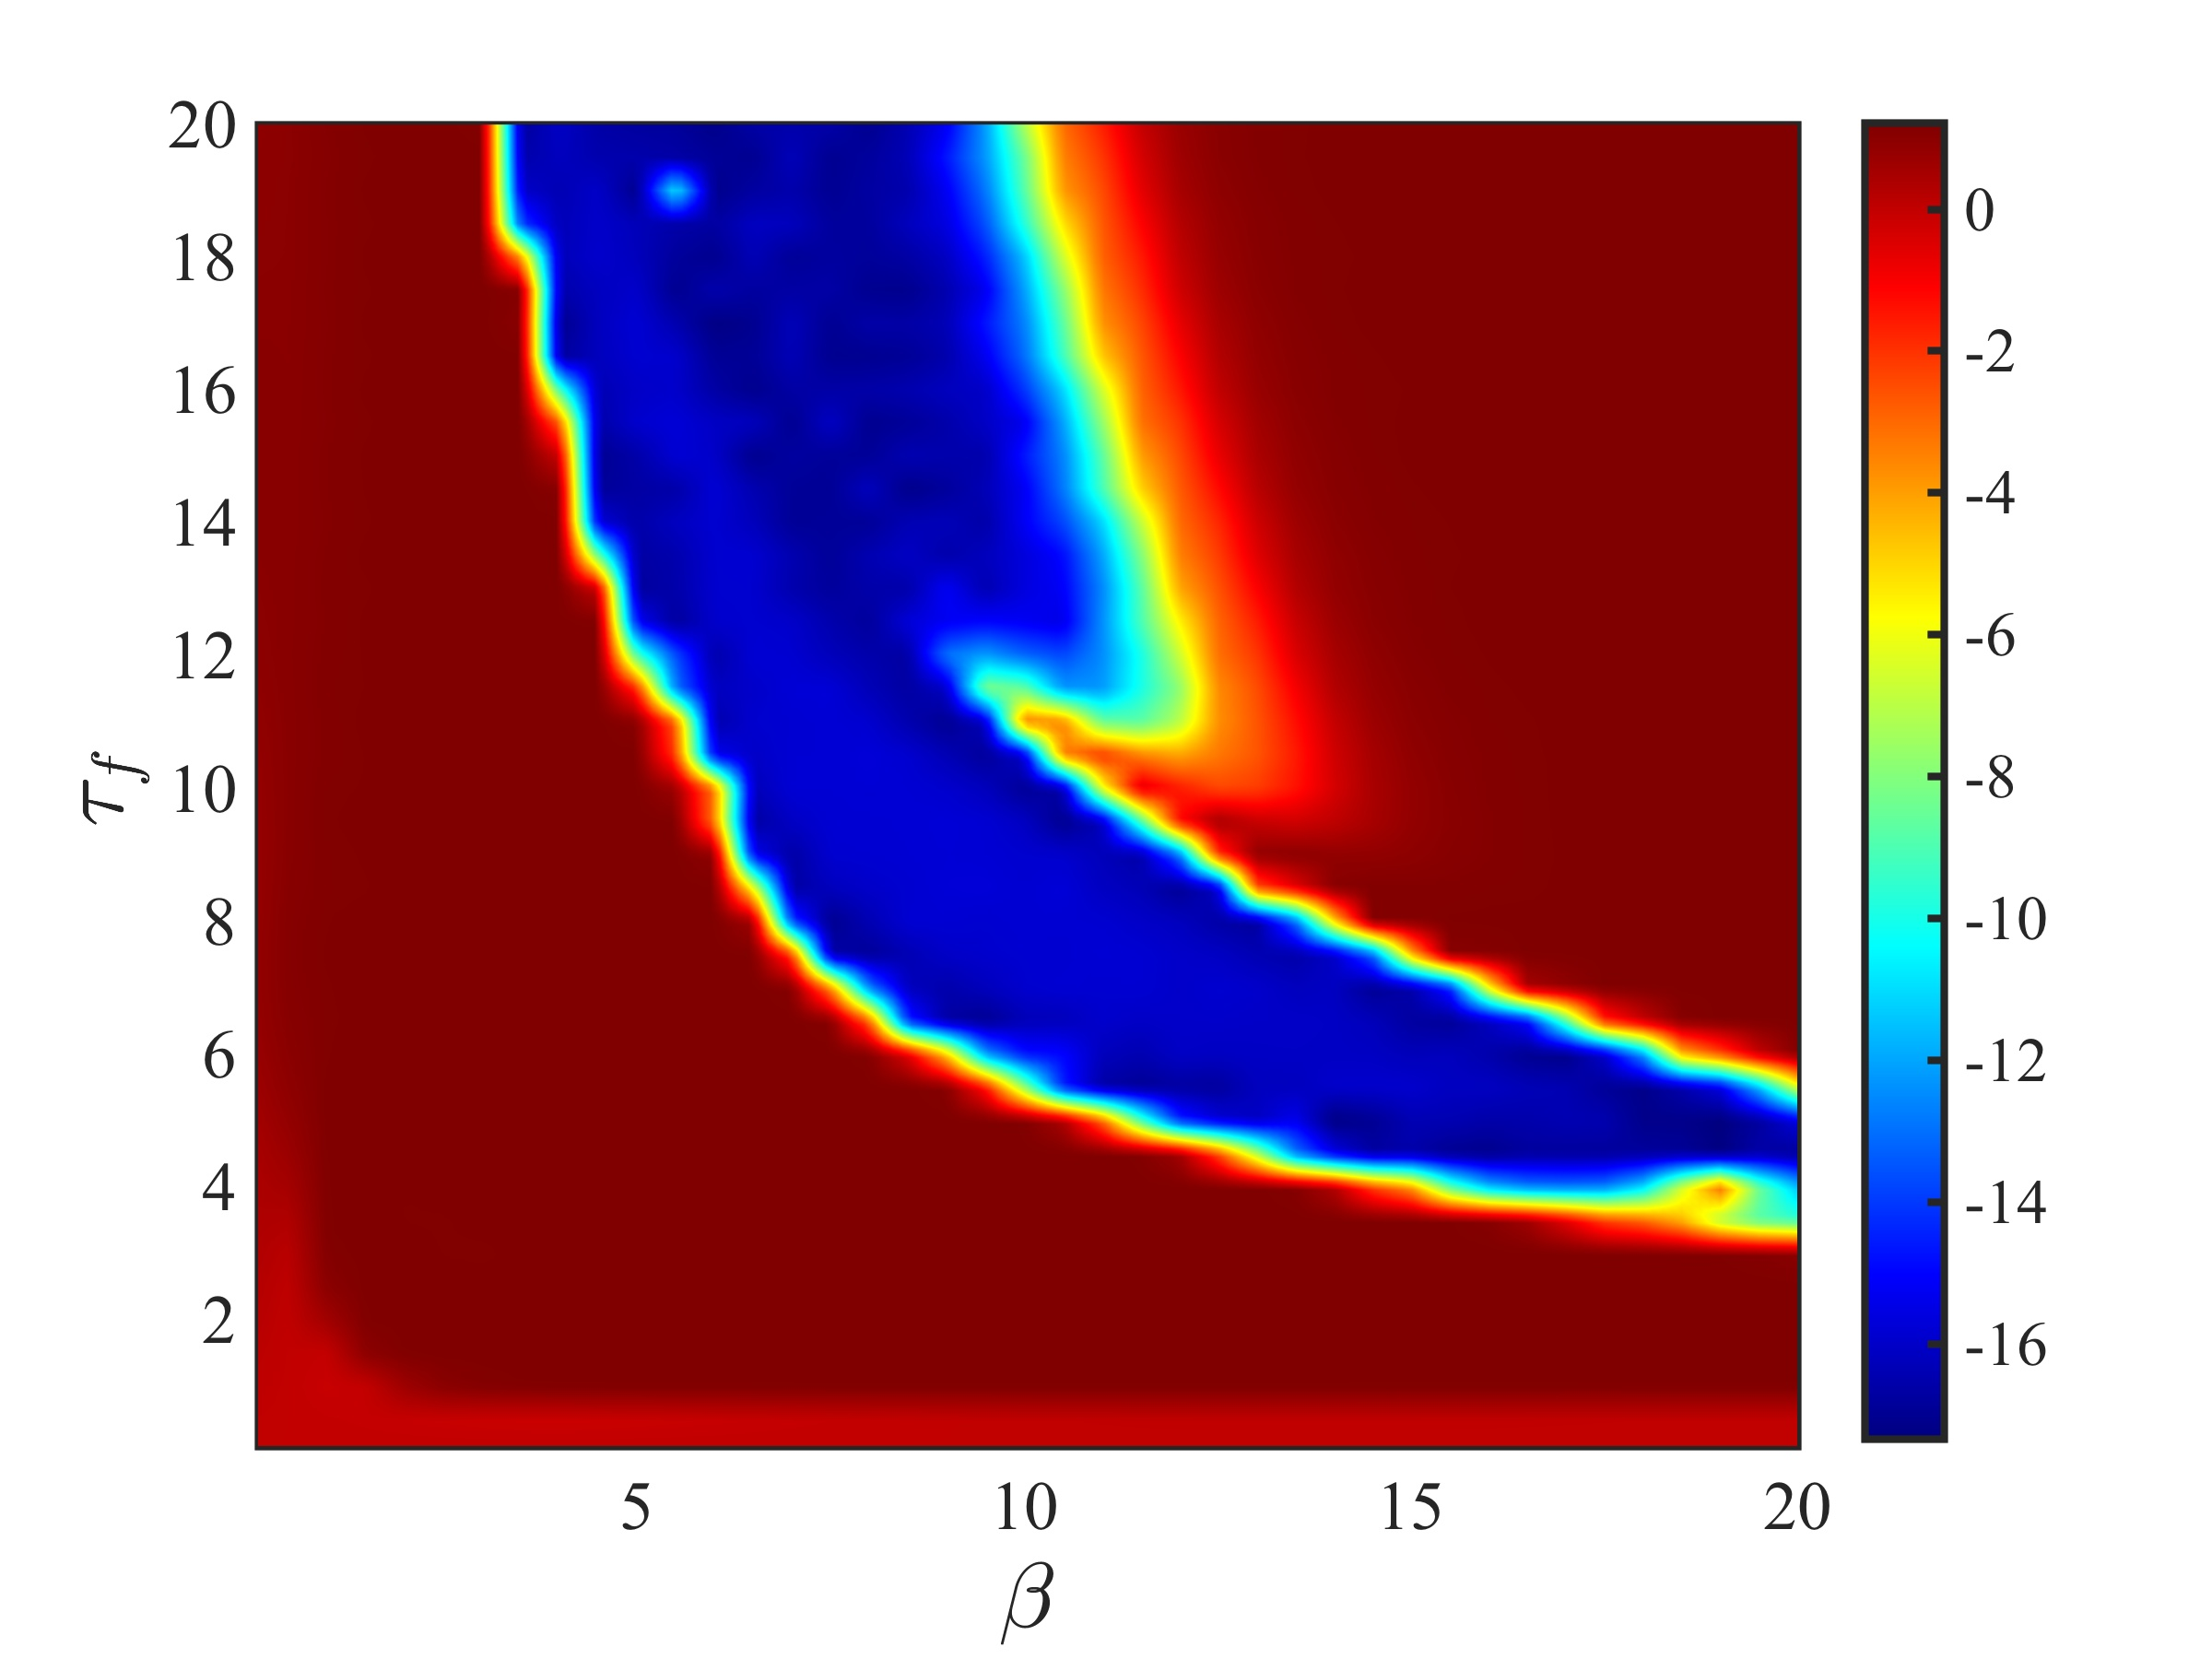
\includegraphics[width=\linewidth]{ACSkinnyQIn.jpg}
\caption{} 
\end{subfigure}
%\hspace*{\fill}
\hspace*{-0.5cm}
\begin{subfigure}{0.5\textwidth}
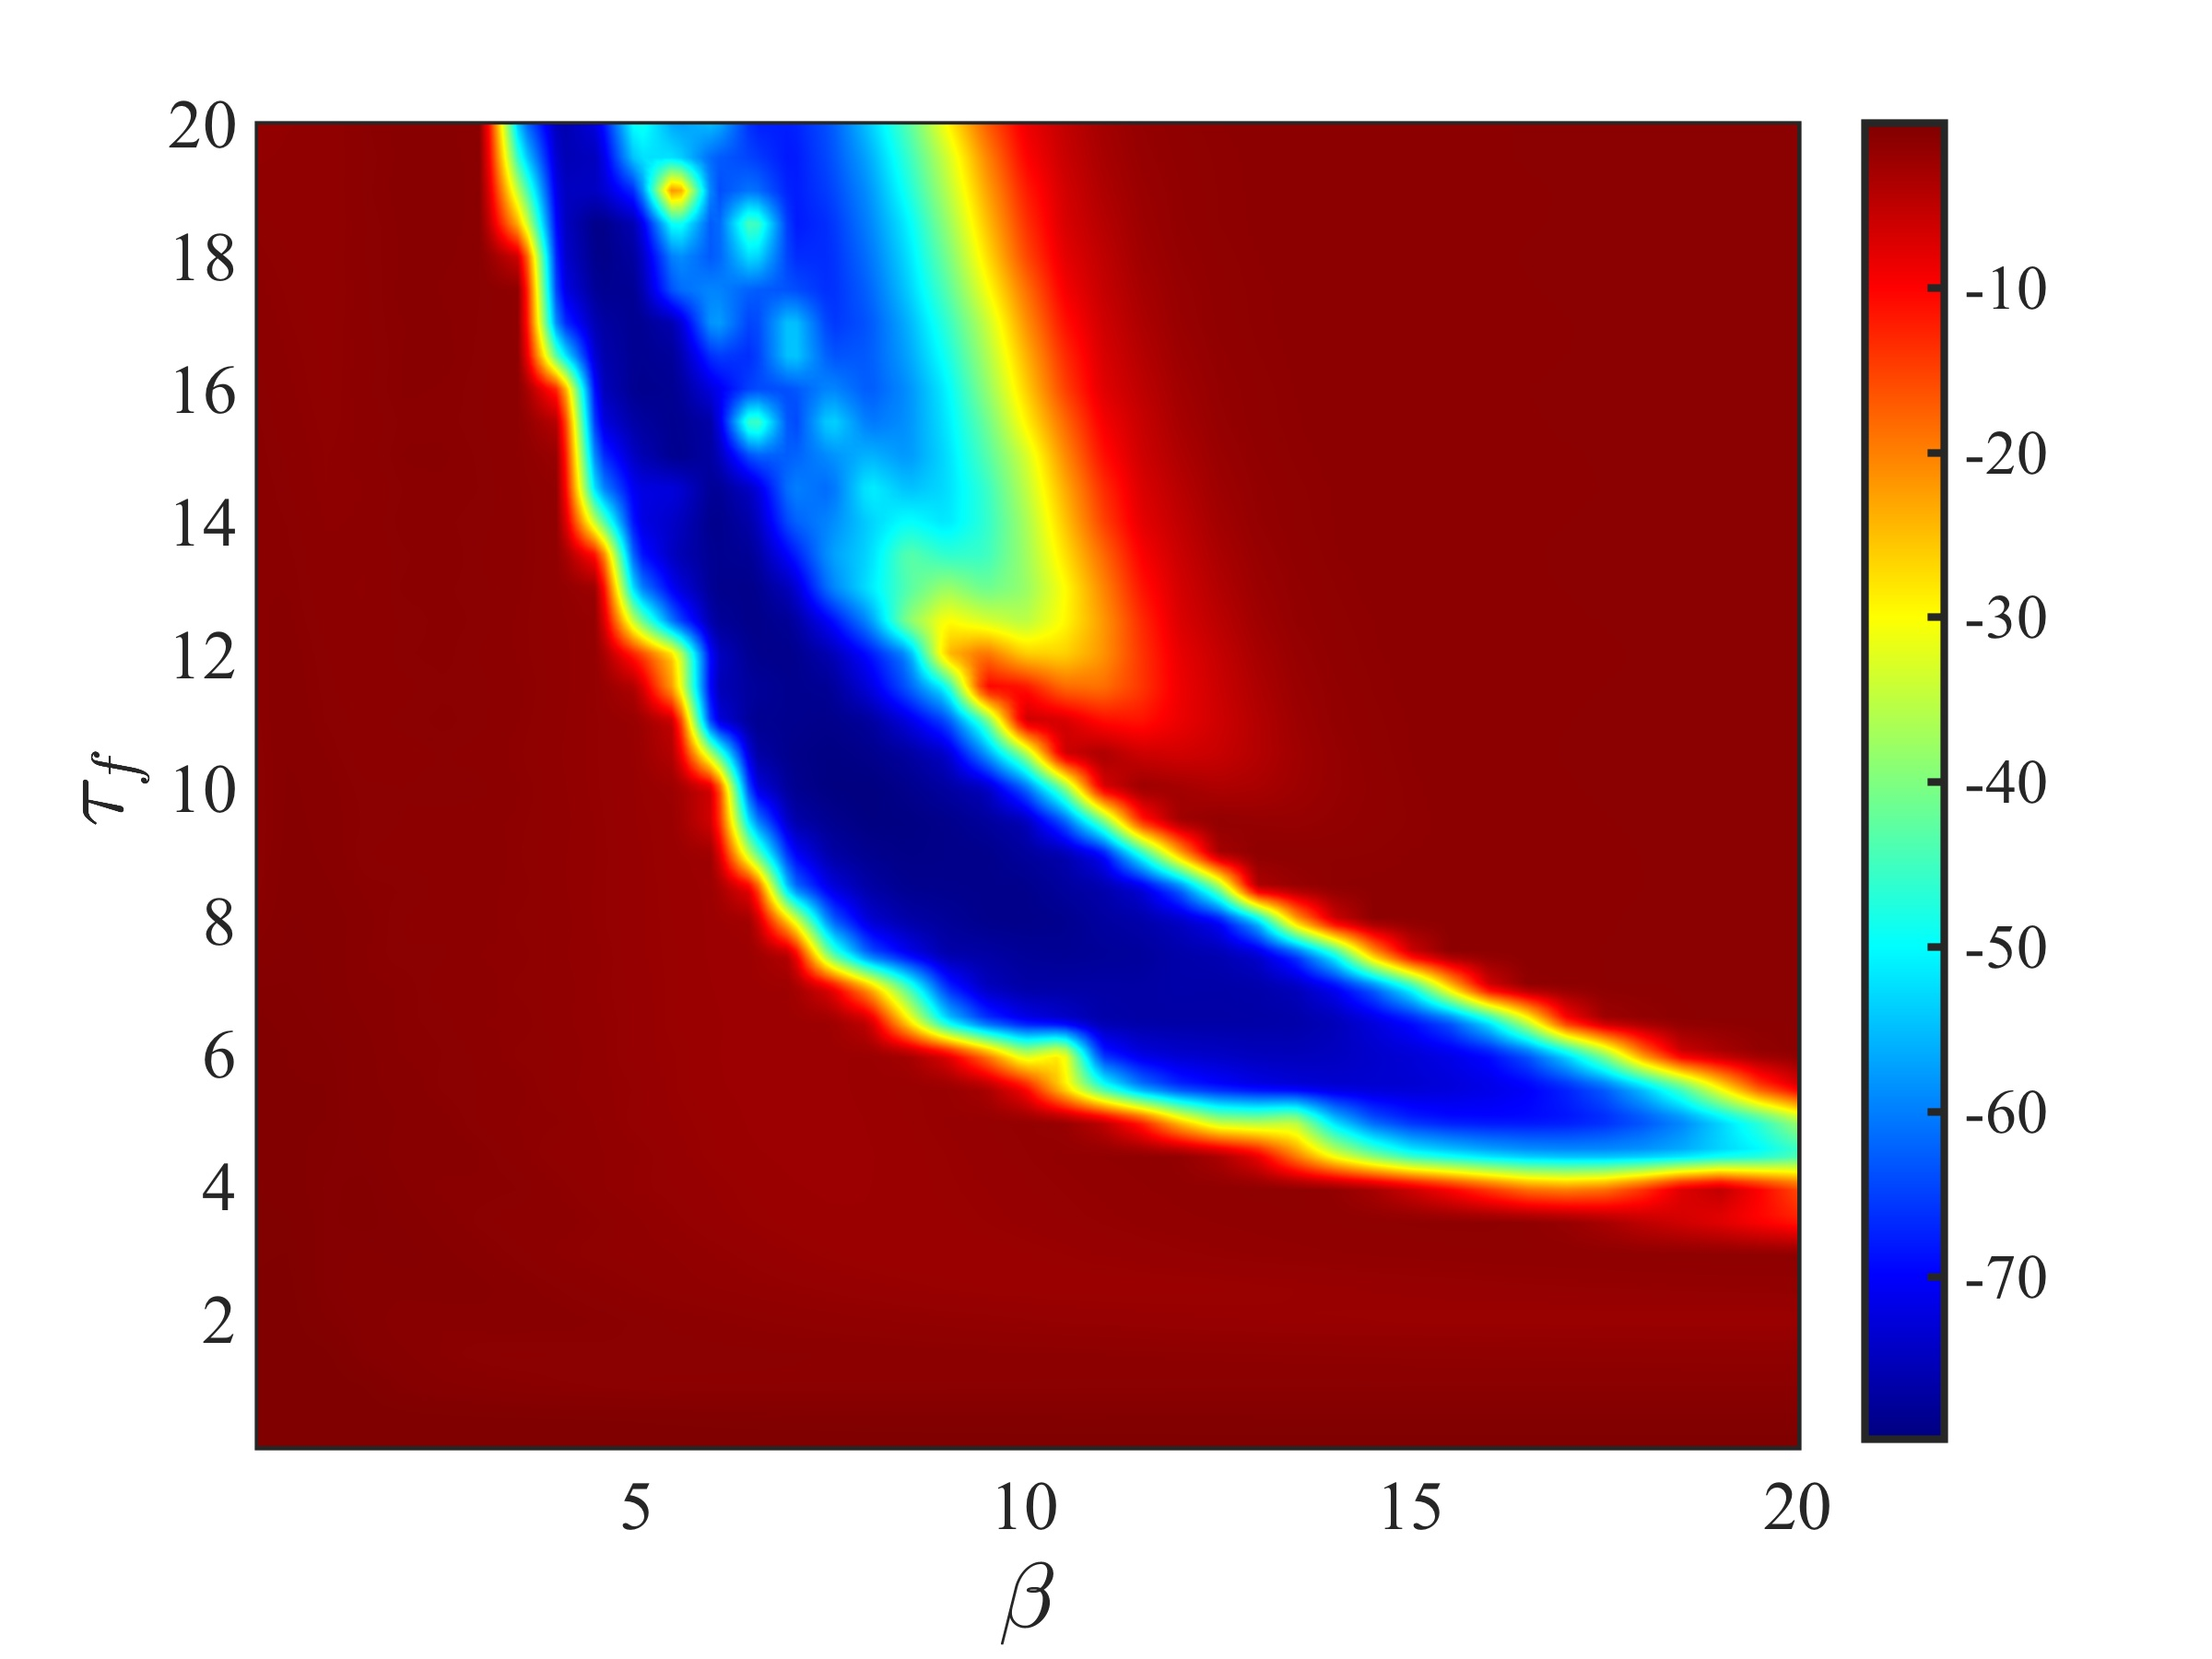
\includegraphics[width=\linewidth]{ACSkinnyQOut.jpg} 
\caption{} 
\end{subfigure} 
\centerline{
%\hspace{1cm}
\begin{subfigure}{\textwidth}
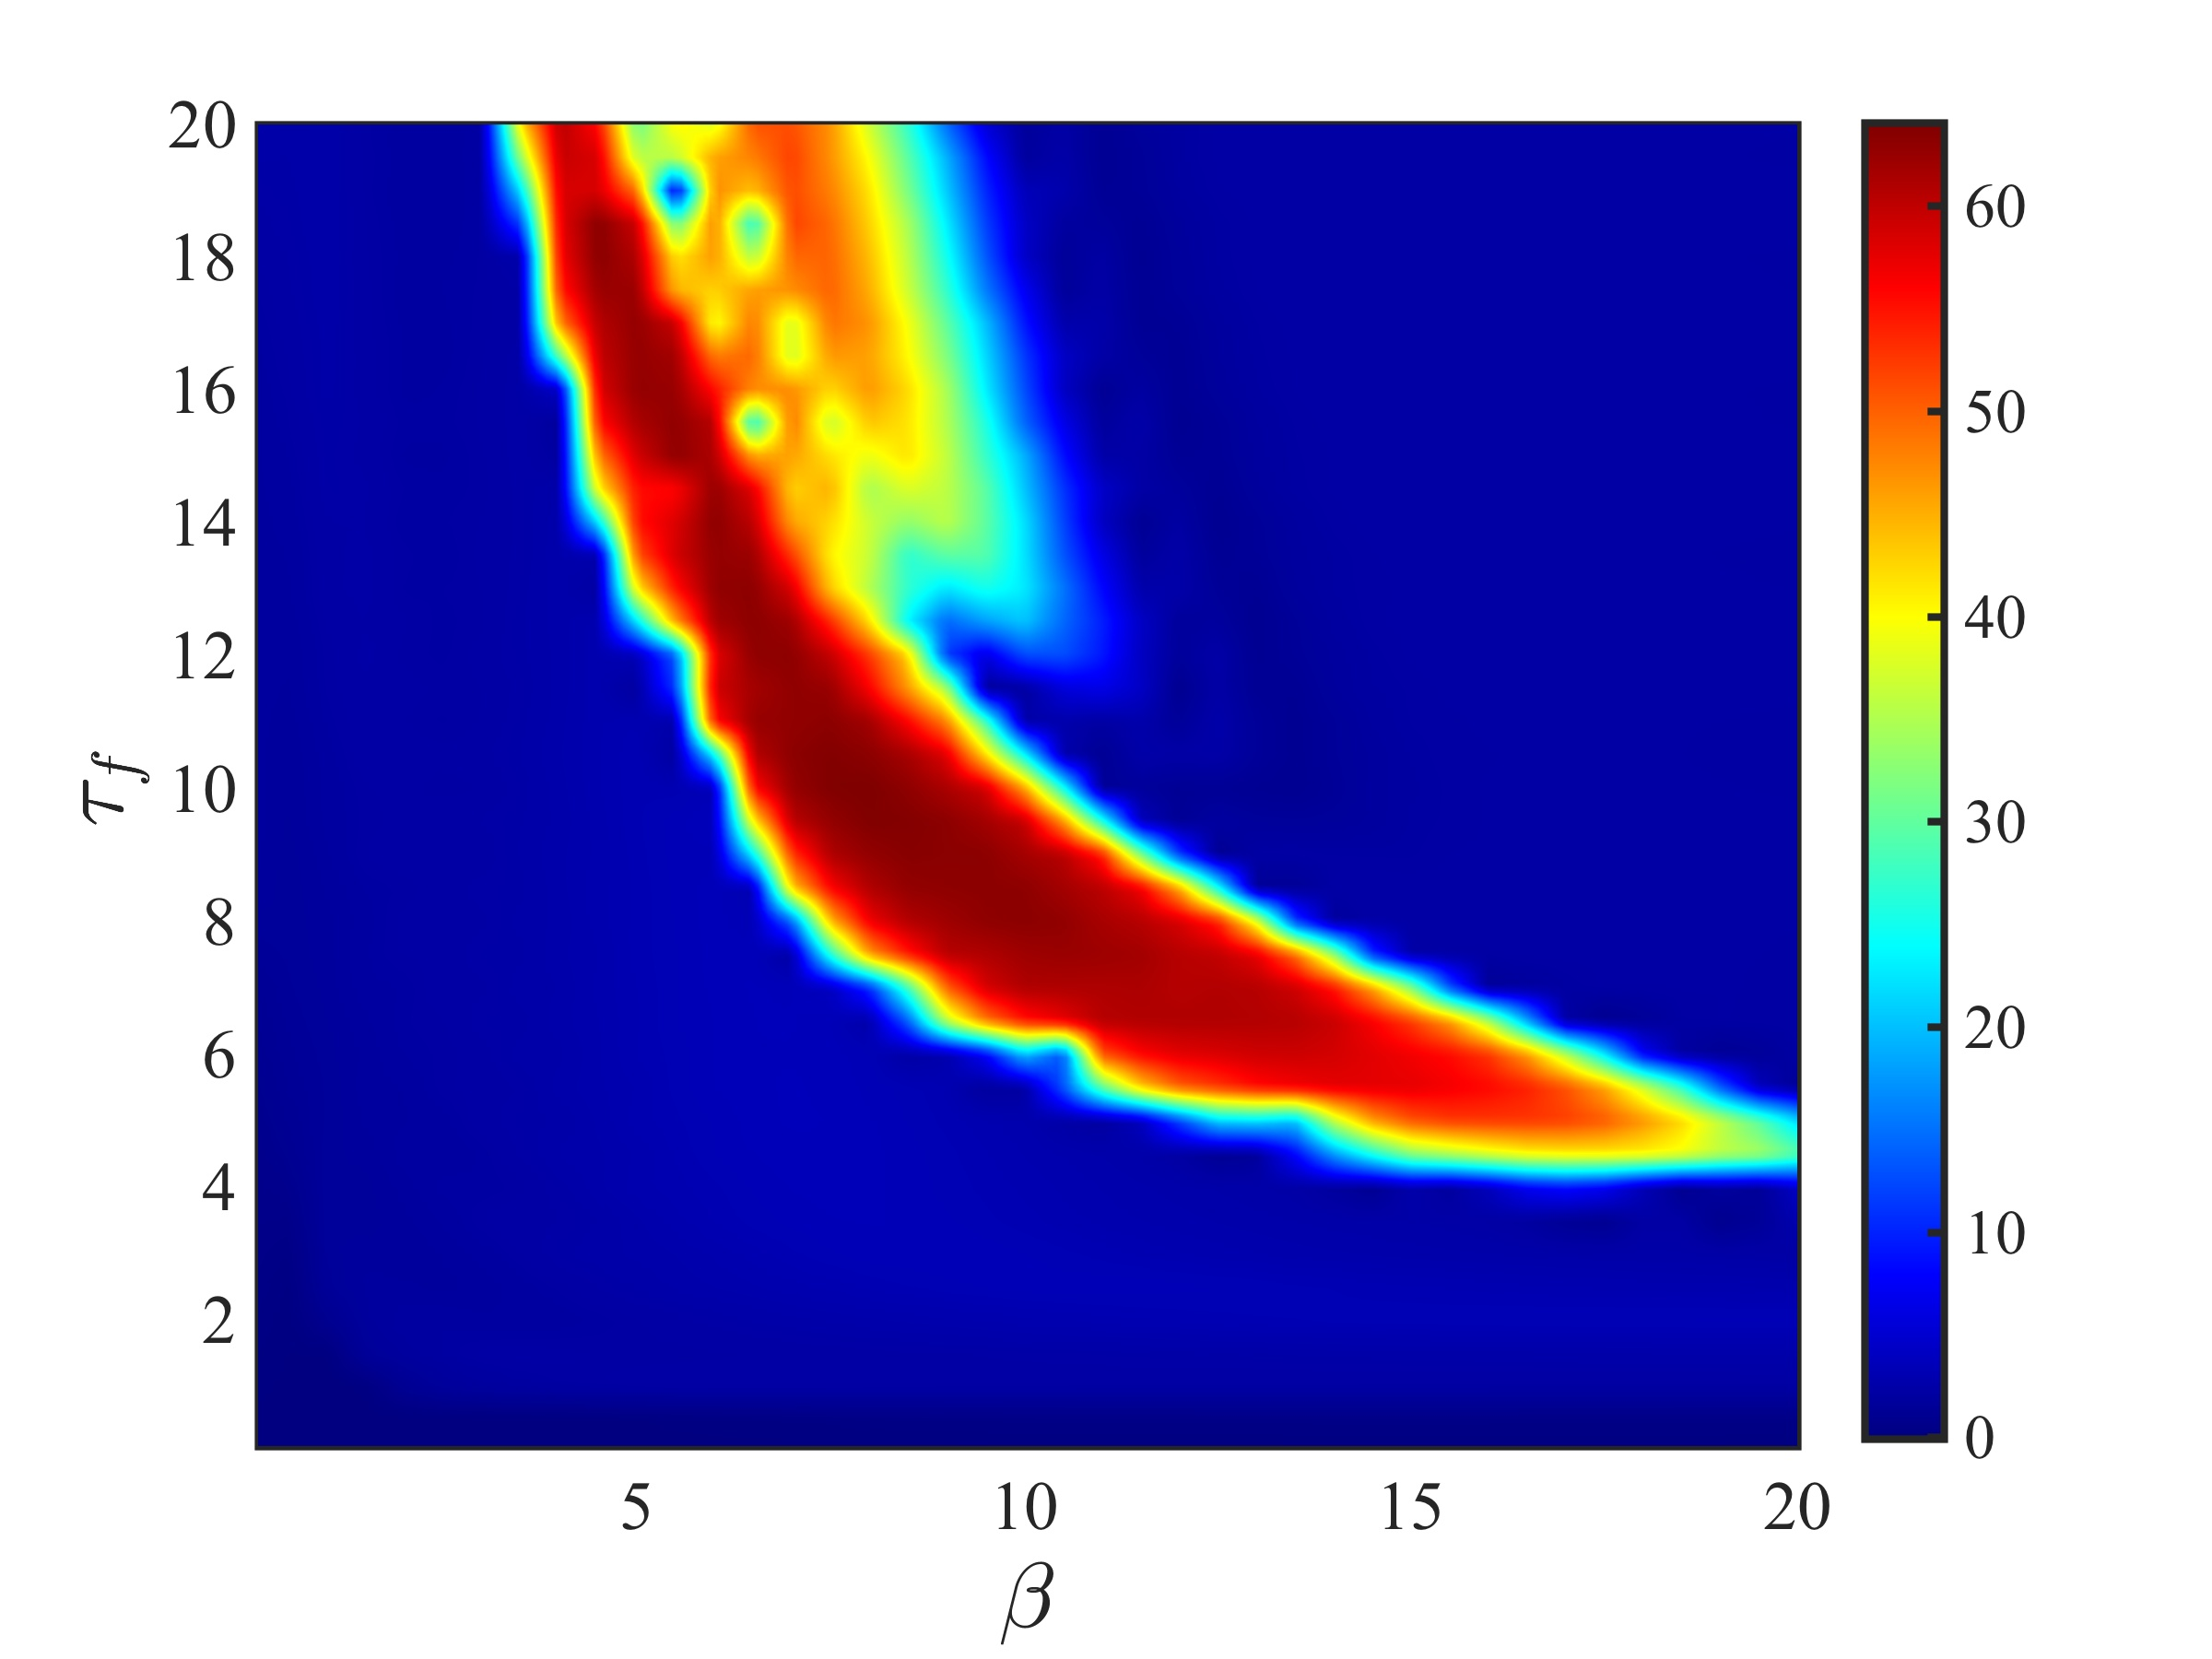
\includegraphics[width=\linewidth]{ACSkinnyQDiff.jpg} 
\caption{} 
\end{subfigure} }
  \rule{35em}{0.5pt}
\caption[Power Ratios Inside and Outside Tweezer with $\sigma_\phi = 0.5$ and $h_\phi = 2$]{
The density of the power ratios (a) inside and (b) outside of a narrow tweezer width $\sigma_\phi = 0.5$ and height $h_\phi = 2$.  The detuning for the system is $\Delta =  2.8074$ and each combination of parameter is evolved for $z_f = 10 = 4z^*$, with $z^* = 2.5$.  (a) The power ratio density inside the tweezer $Q_{\rm I}$, where blue ($Q_{\rm I}=0$) is complete power inside the tweezer at $z_f$ and red ($Q_{\rm I}=1$) is no power inside the tweezer at $z_f$.  (b) The power ratio density outside the tweezer $Q_{\rm O}$, where $Q_{\rm O}$ = 0 depicts no change in power.  (c) The difference in power ratios inside and outside the tweezer, $Q_{\rm I} - Q_{\rm O}$.  The difference between the power ratios (c) defines the thresholds for tweezed CSs for all blue regions, no-CSs for all green regions, and non-tweezed CSs for all red regions.  
}
\label{fig:ACSkinnyQ}
\end{figure}

Figure~\ref{fig:ACRegularQ} depicts the density of the power ratios inside $Q_{\rm I}$ (top) and outside $Q_{\rm O}$ (bottom) of a tweezer with width $\sigma_\phi = 1$ and $h_\phi = 2$.  For the full LL Eq.~(\ref{eq:LLETweeze}) with $u_{\rm in} = 2$, the steady state CS is found centered at $\tau_0 = 0$ using a Newton-Krylov solver and the power-balance constraint Eq.~(\ref{LLConstraint}) which selects a particular detuning parameter $\Delta =  3.1488$ for the system.  
\begin{figure}[htb!]
\centering
\hspace{0cm}
\begin{subfigure}{0.5\textwidth}
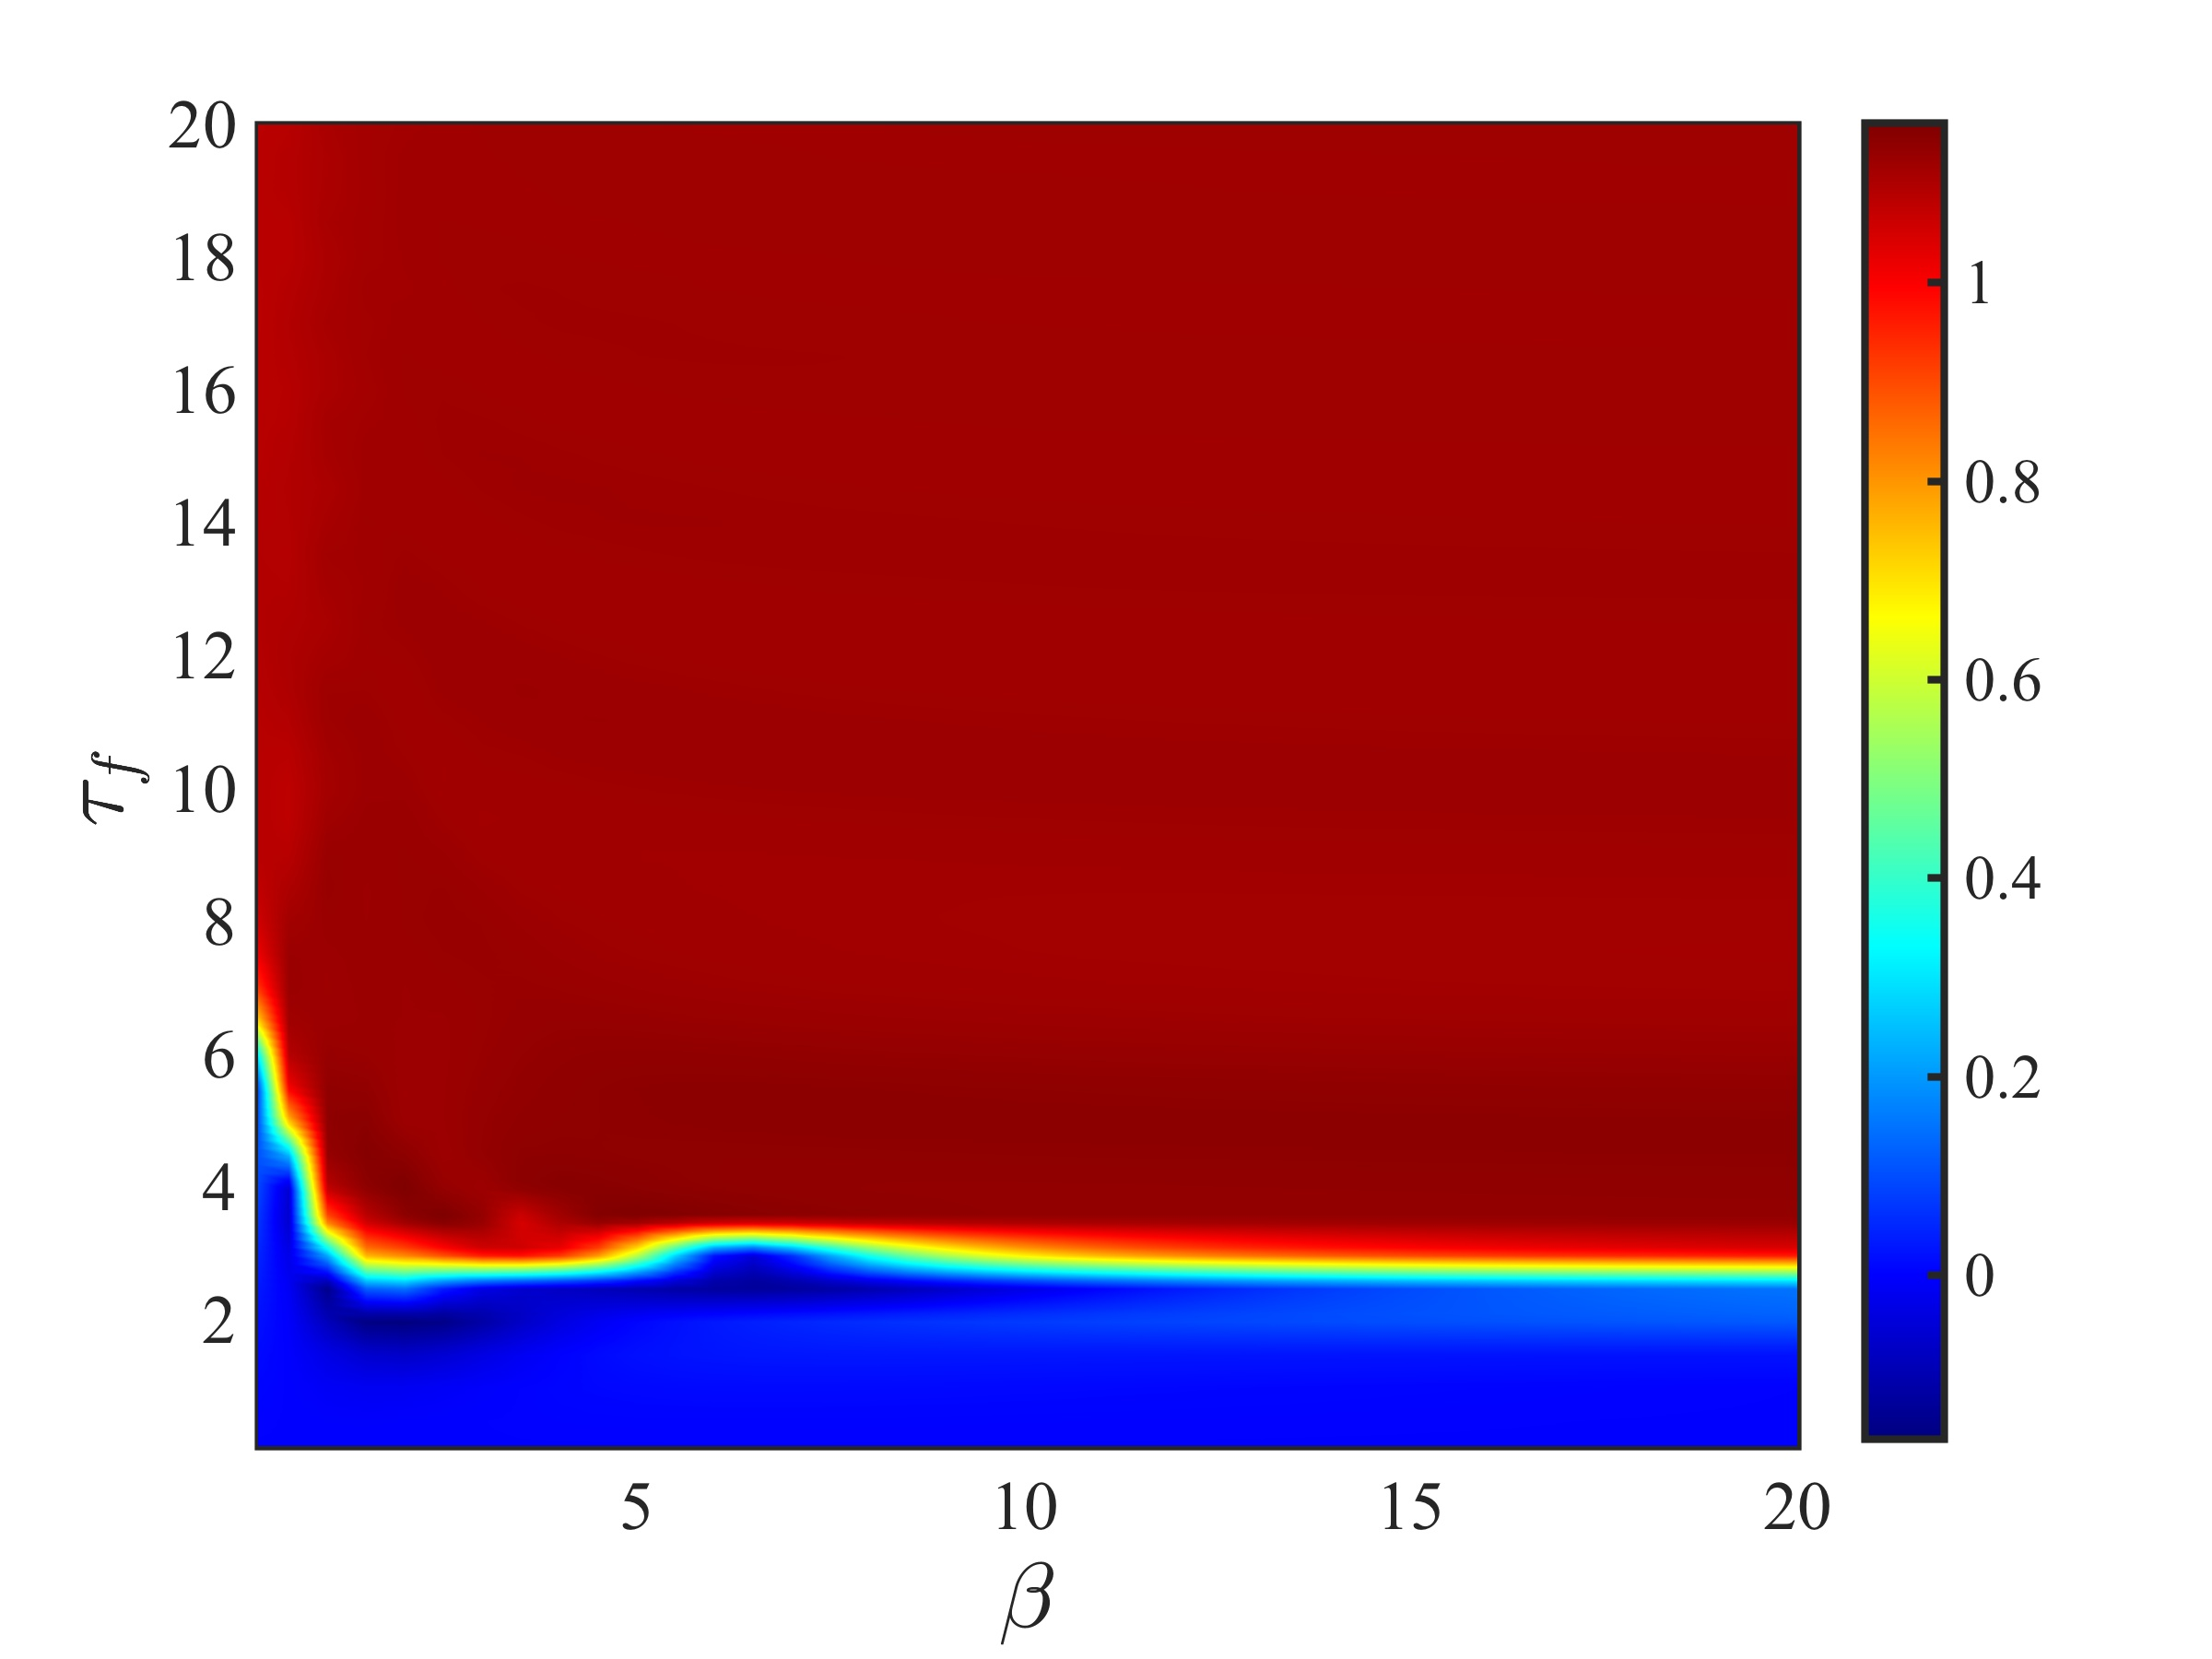
\includegraphics[width=\linewidth]{ACRegularQIn.jpg}
\caption{} 
\end{subfigure}
%\hspace*{\fill}
\hspace*{-0.5cm}
\begin{subfigure}{0.5\textwidth}
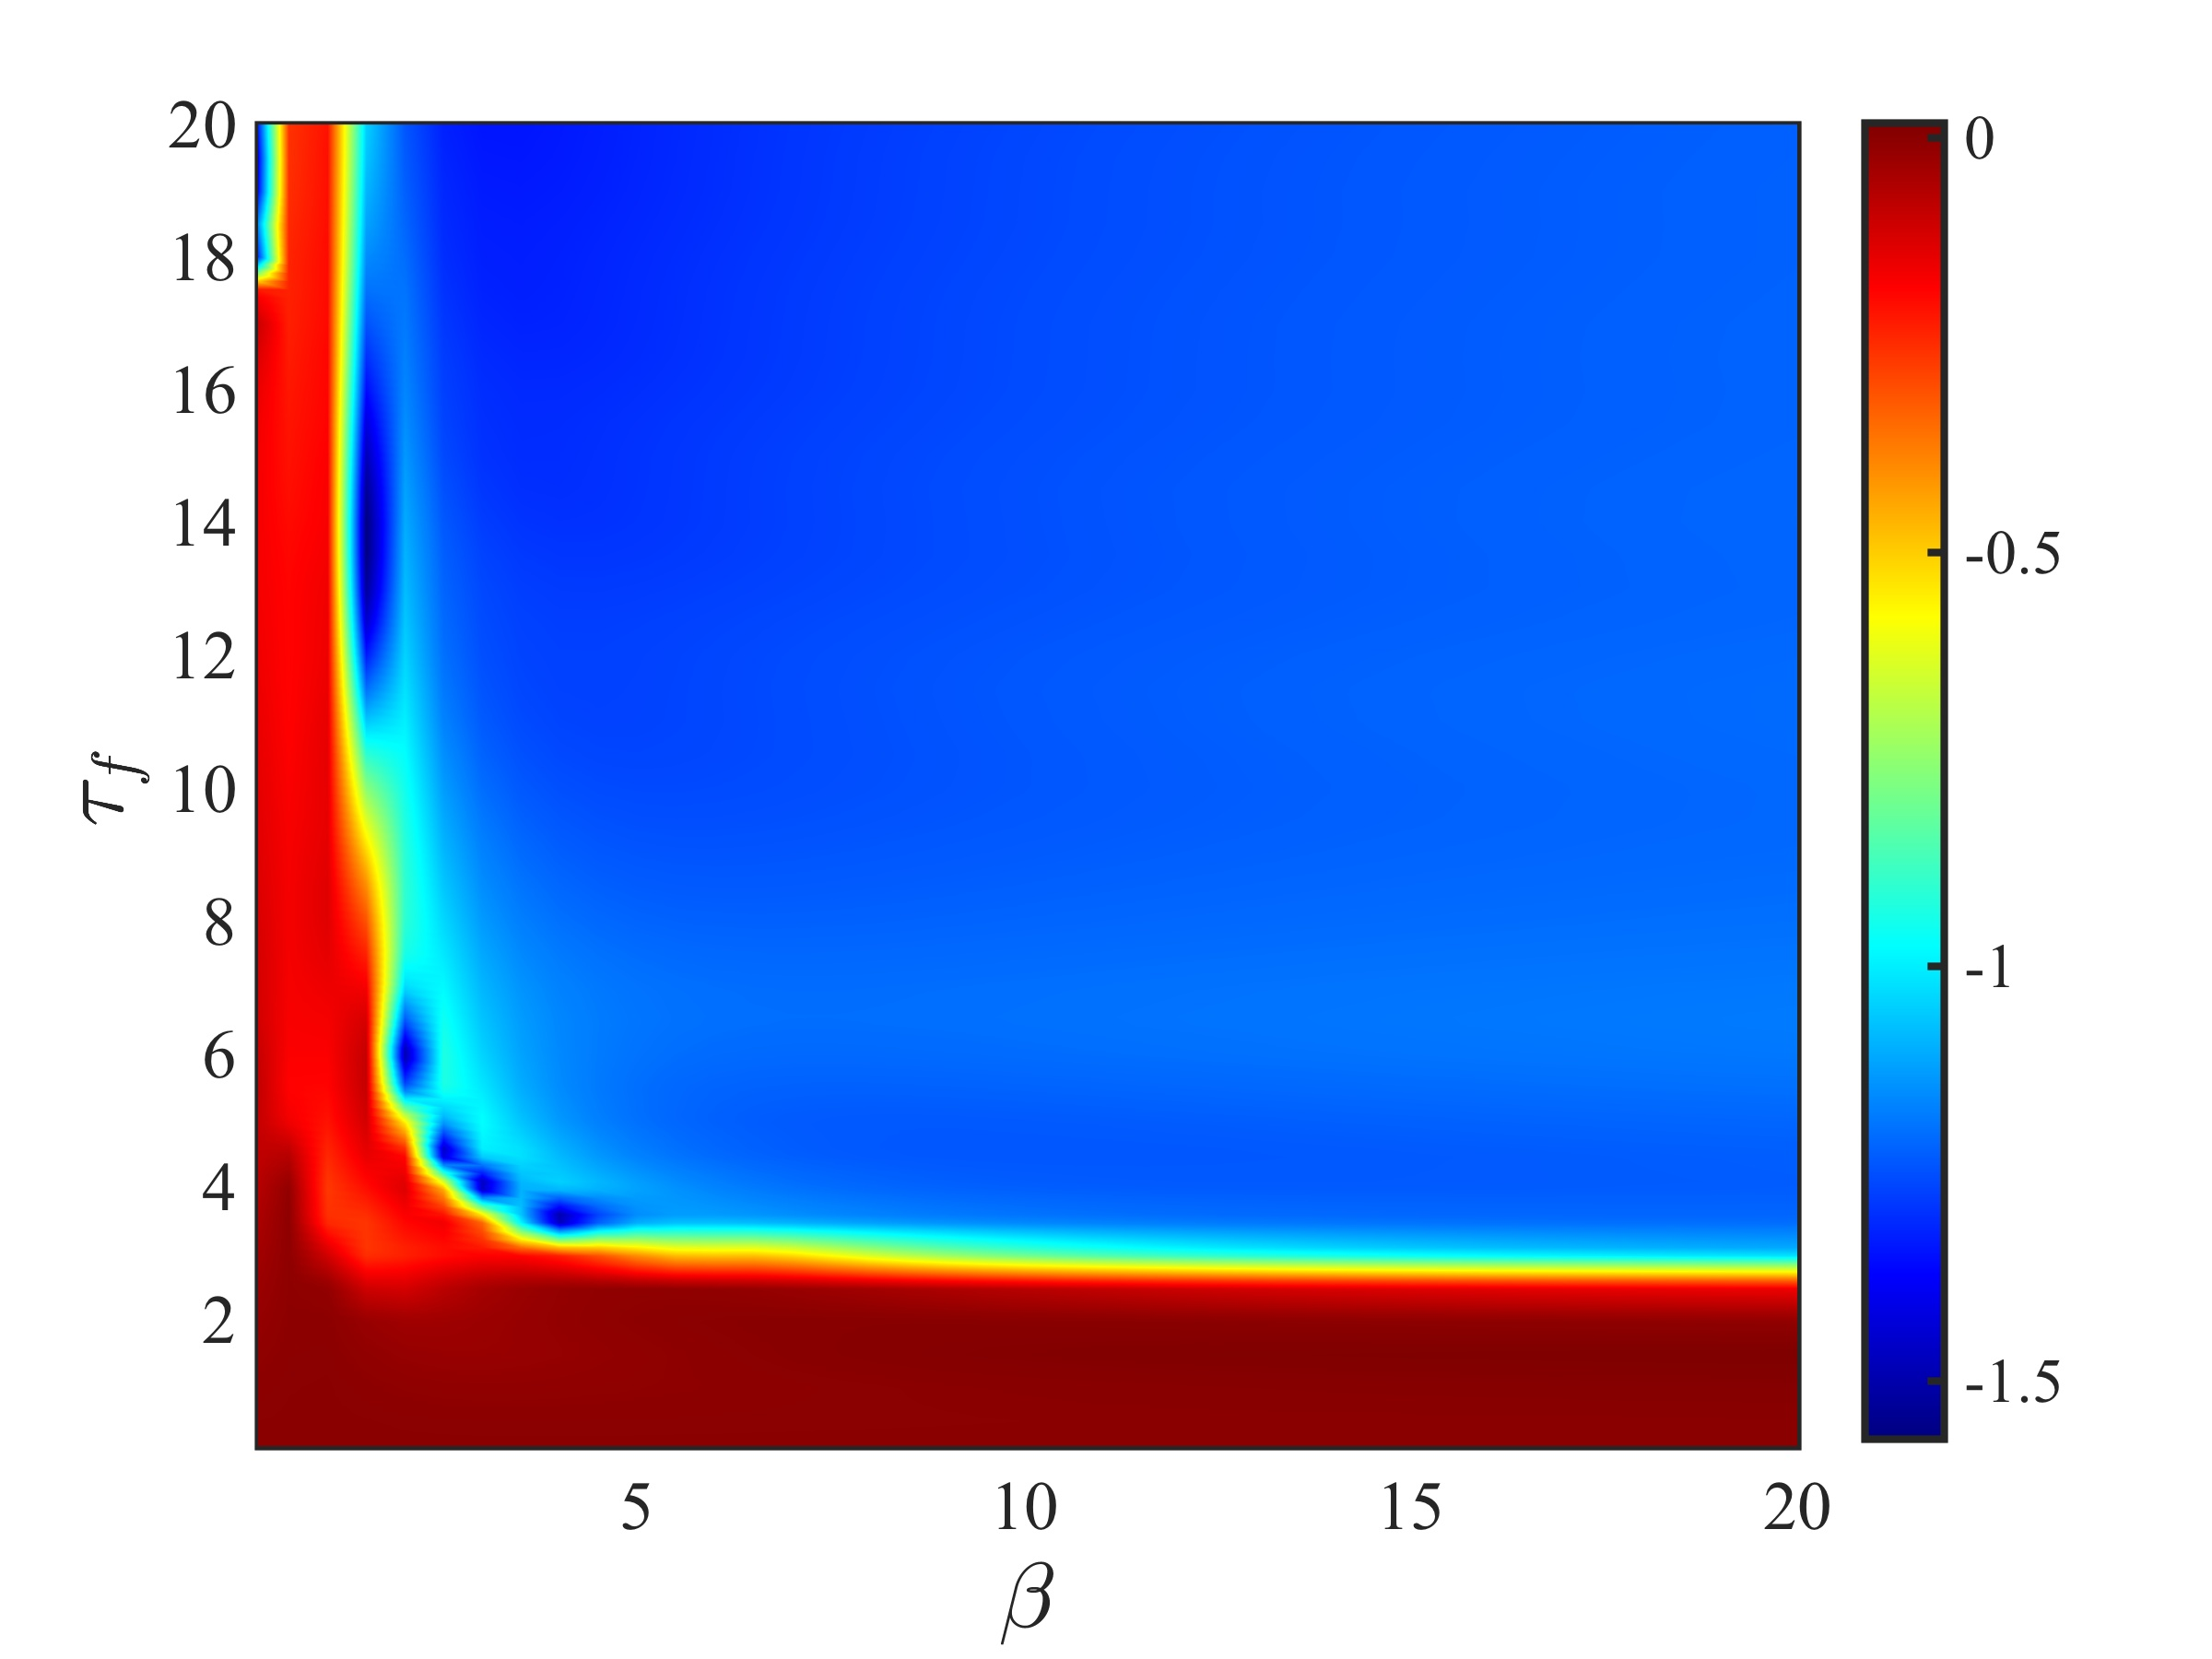
\includegraphics[width=\linewidth]{ACRegularQOut.jpg} 
\caption{} 
\end{subfigure} 
\centerline{
%\hspace{1cm}
\begin{subfigure}{\textwidth}
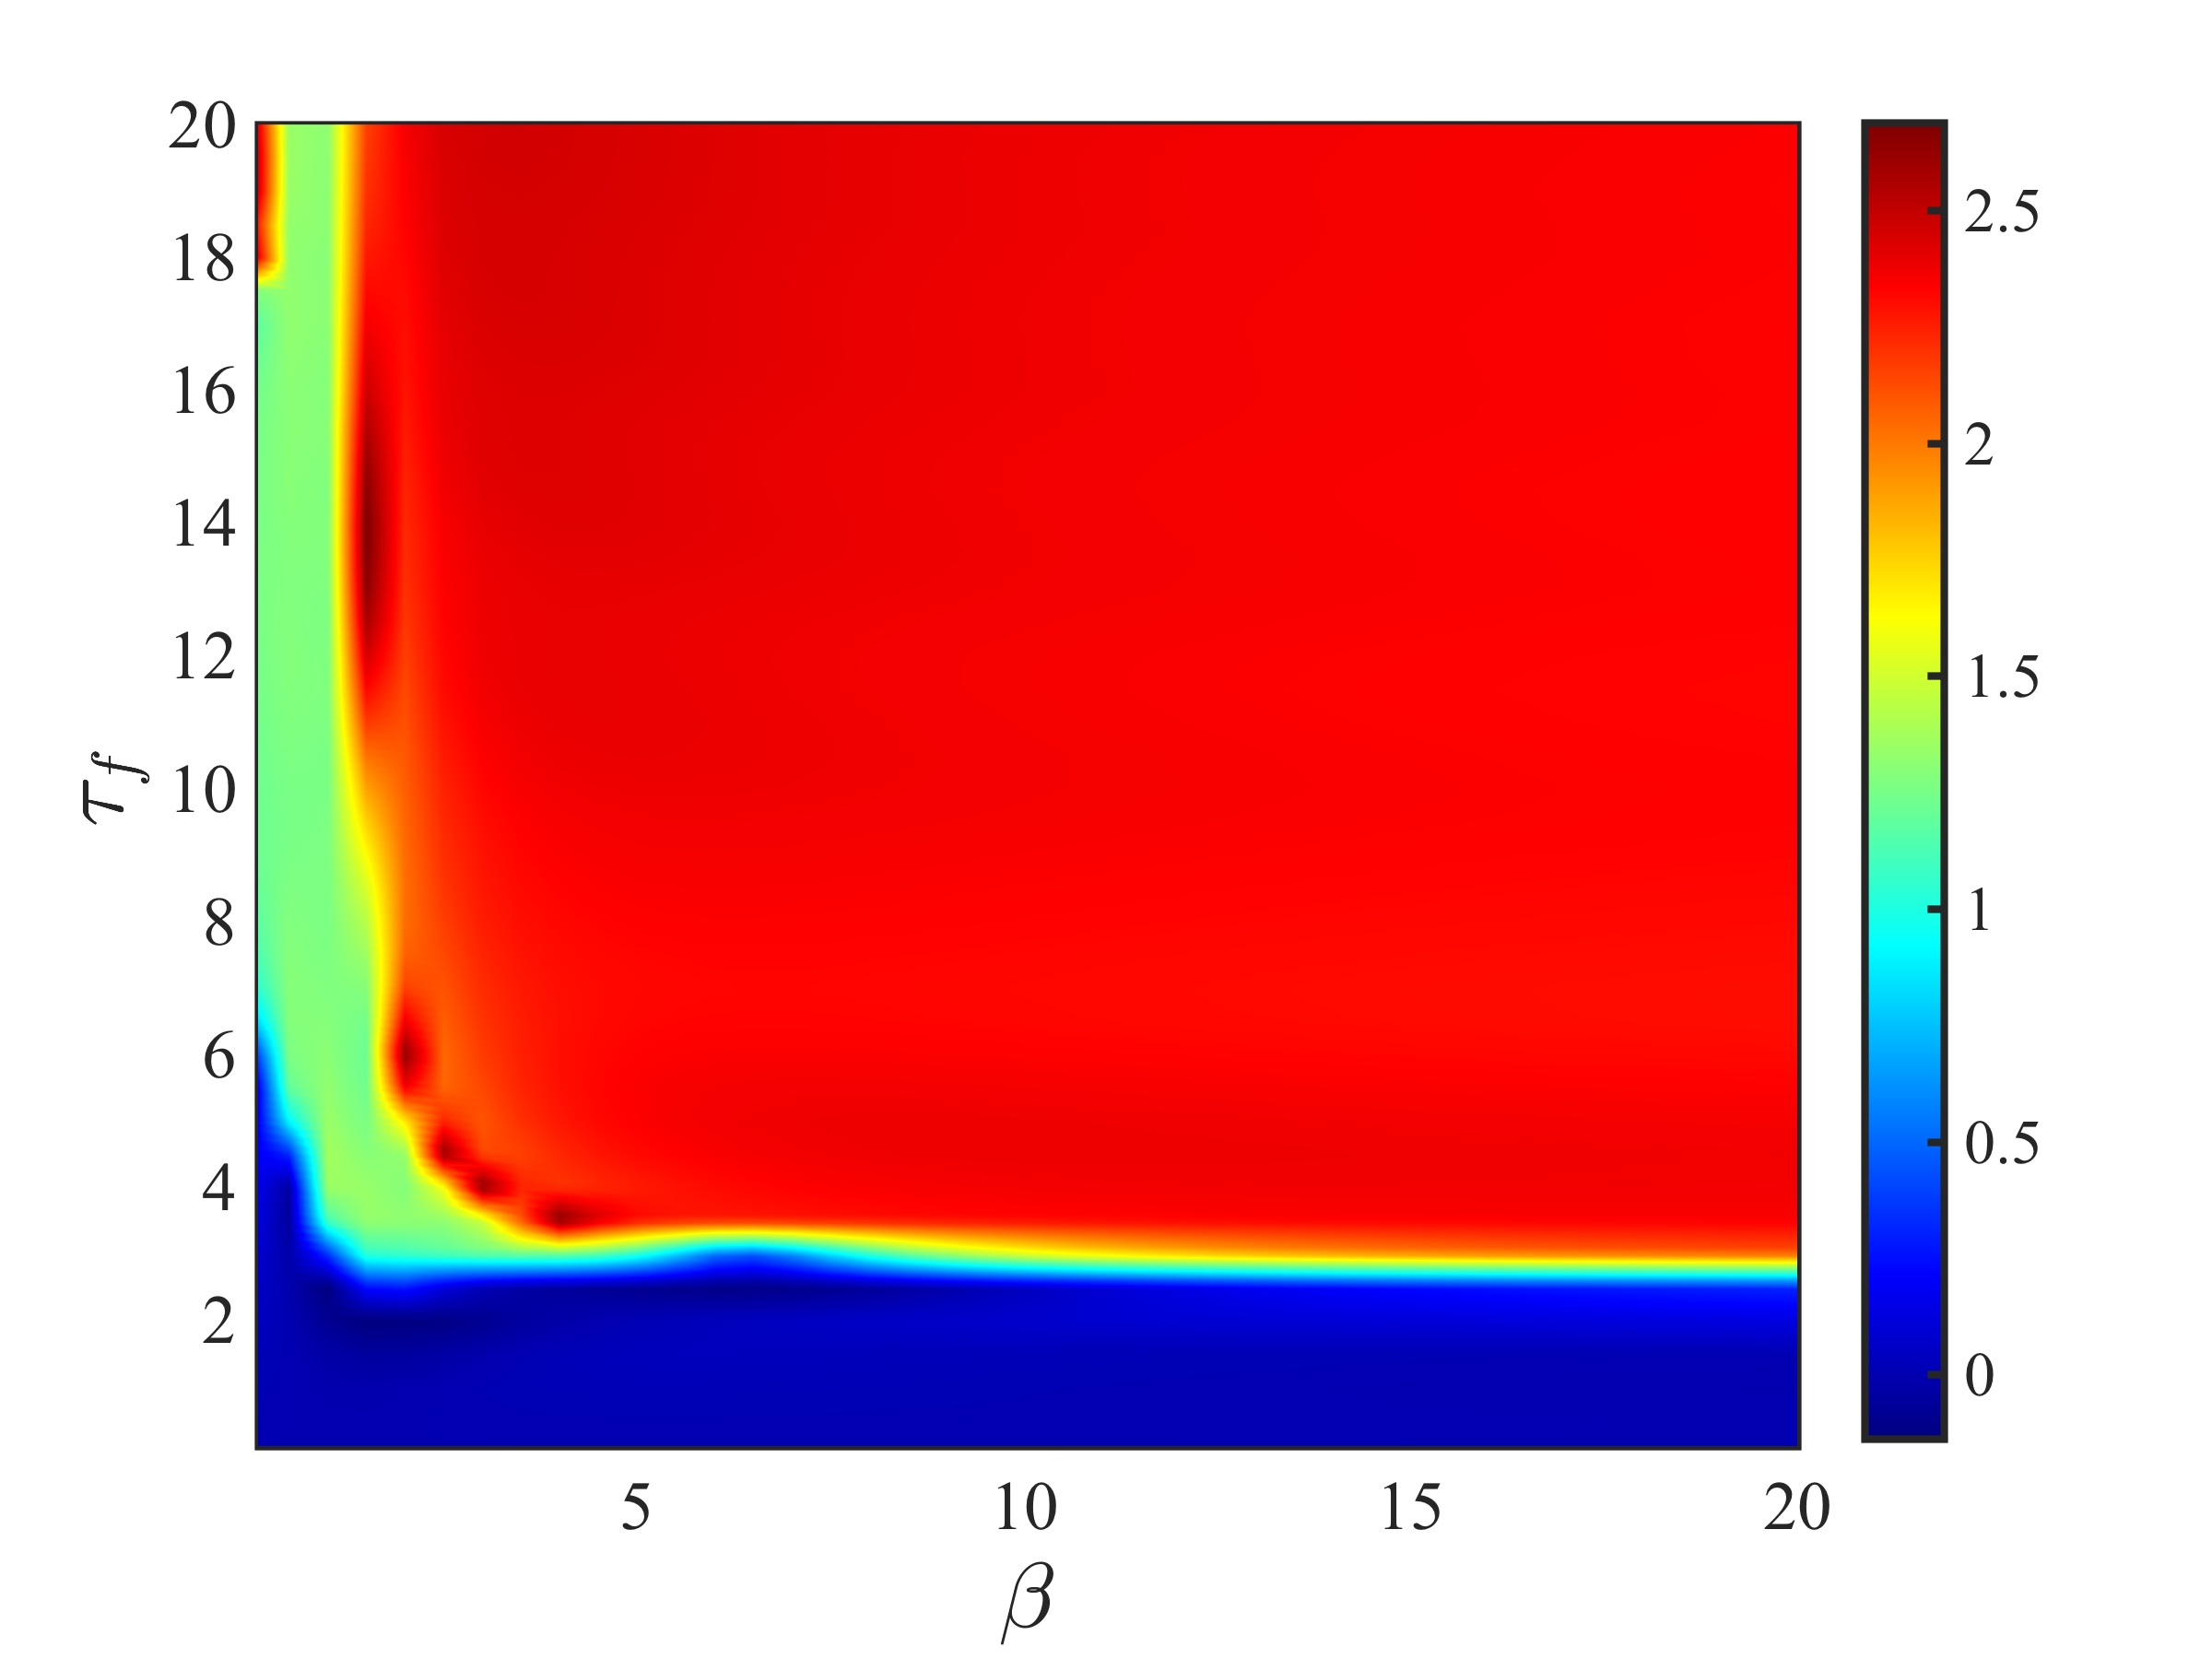
\includegraphics[width=\linewidth]{ACRegularQDiff.jpg} 
\caption{} 
\end{subfigure} }
  \rule{35em}{0.5pt}
\caption[Power Ratios Inside and Outside Tweezer with $\sigma_\phi = 1$ and $h_\phi = 2$]{
Power ratios as in Fig.~\ref{fig:ACSkinnyQ} but for a  tweezer with width $\sigma_\phi = 1$ and height $h_\phi = 2$.  The detuning for the system is $\Delta =  3.1488$.   Same layout as in Fig.~\ref{fig:ACSkinnyQ}.  The difference power ratio (c) defines the thresholds for tweezed CSs for all blue regions, no-CSs for all green regions, and non-tweezed CSs for all red regions.  
}
\label{fig:ACRegularQ}
\end{figure}

Figure~\ref{fig:ACFatQ} depicts the density of the power ratios inside $Q_{\rm I}$ (top) and outside $Q_{\rm O}$ (bottom) of a tweezer with width $\sigma_\phi = 2$ and $h_\phi = 2$.  For the full LL Eq.~(\ref{eq:LLETweeze}) with $u_{\rm in} = 2$, the steady state CS is found centered at $\tau_0 = 0$ using a Newton-Krylov solver and the power-balance constraint Eq.~(\ref{LLConstraint}) which selects a detuning parameter $\Delta =  3.3830$ for the system.  The power ratio difference $Q_{\rm diff}$ defines the threshold between the existence of tweezed CSs and no-CSs for most $\beta$ at approximately $\tau_f = 4$.

\begin{figure}[htb!]
\centering
\hspace{0cm}
\begin{subfigure}{0.5\textwidth}
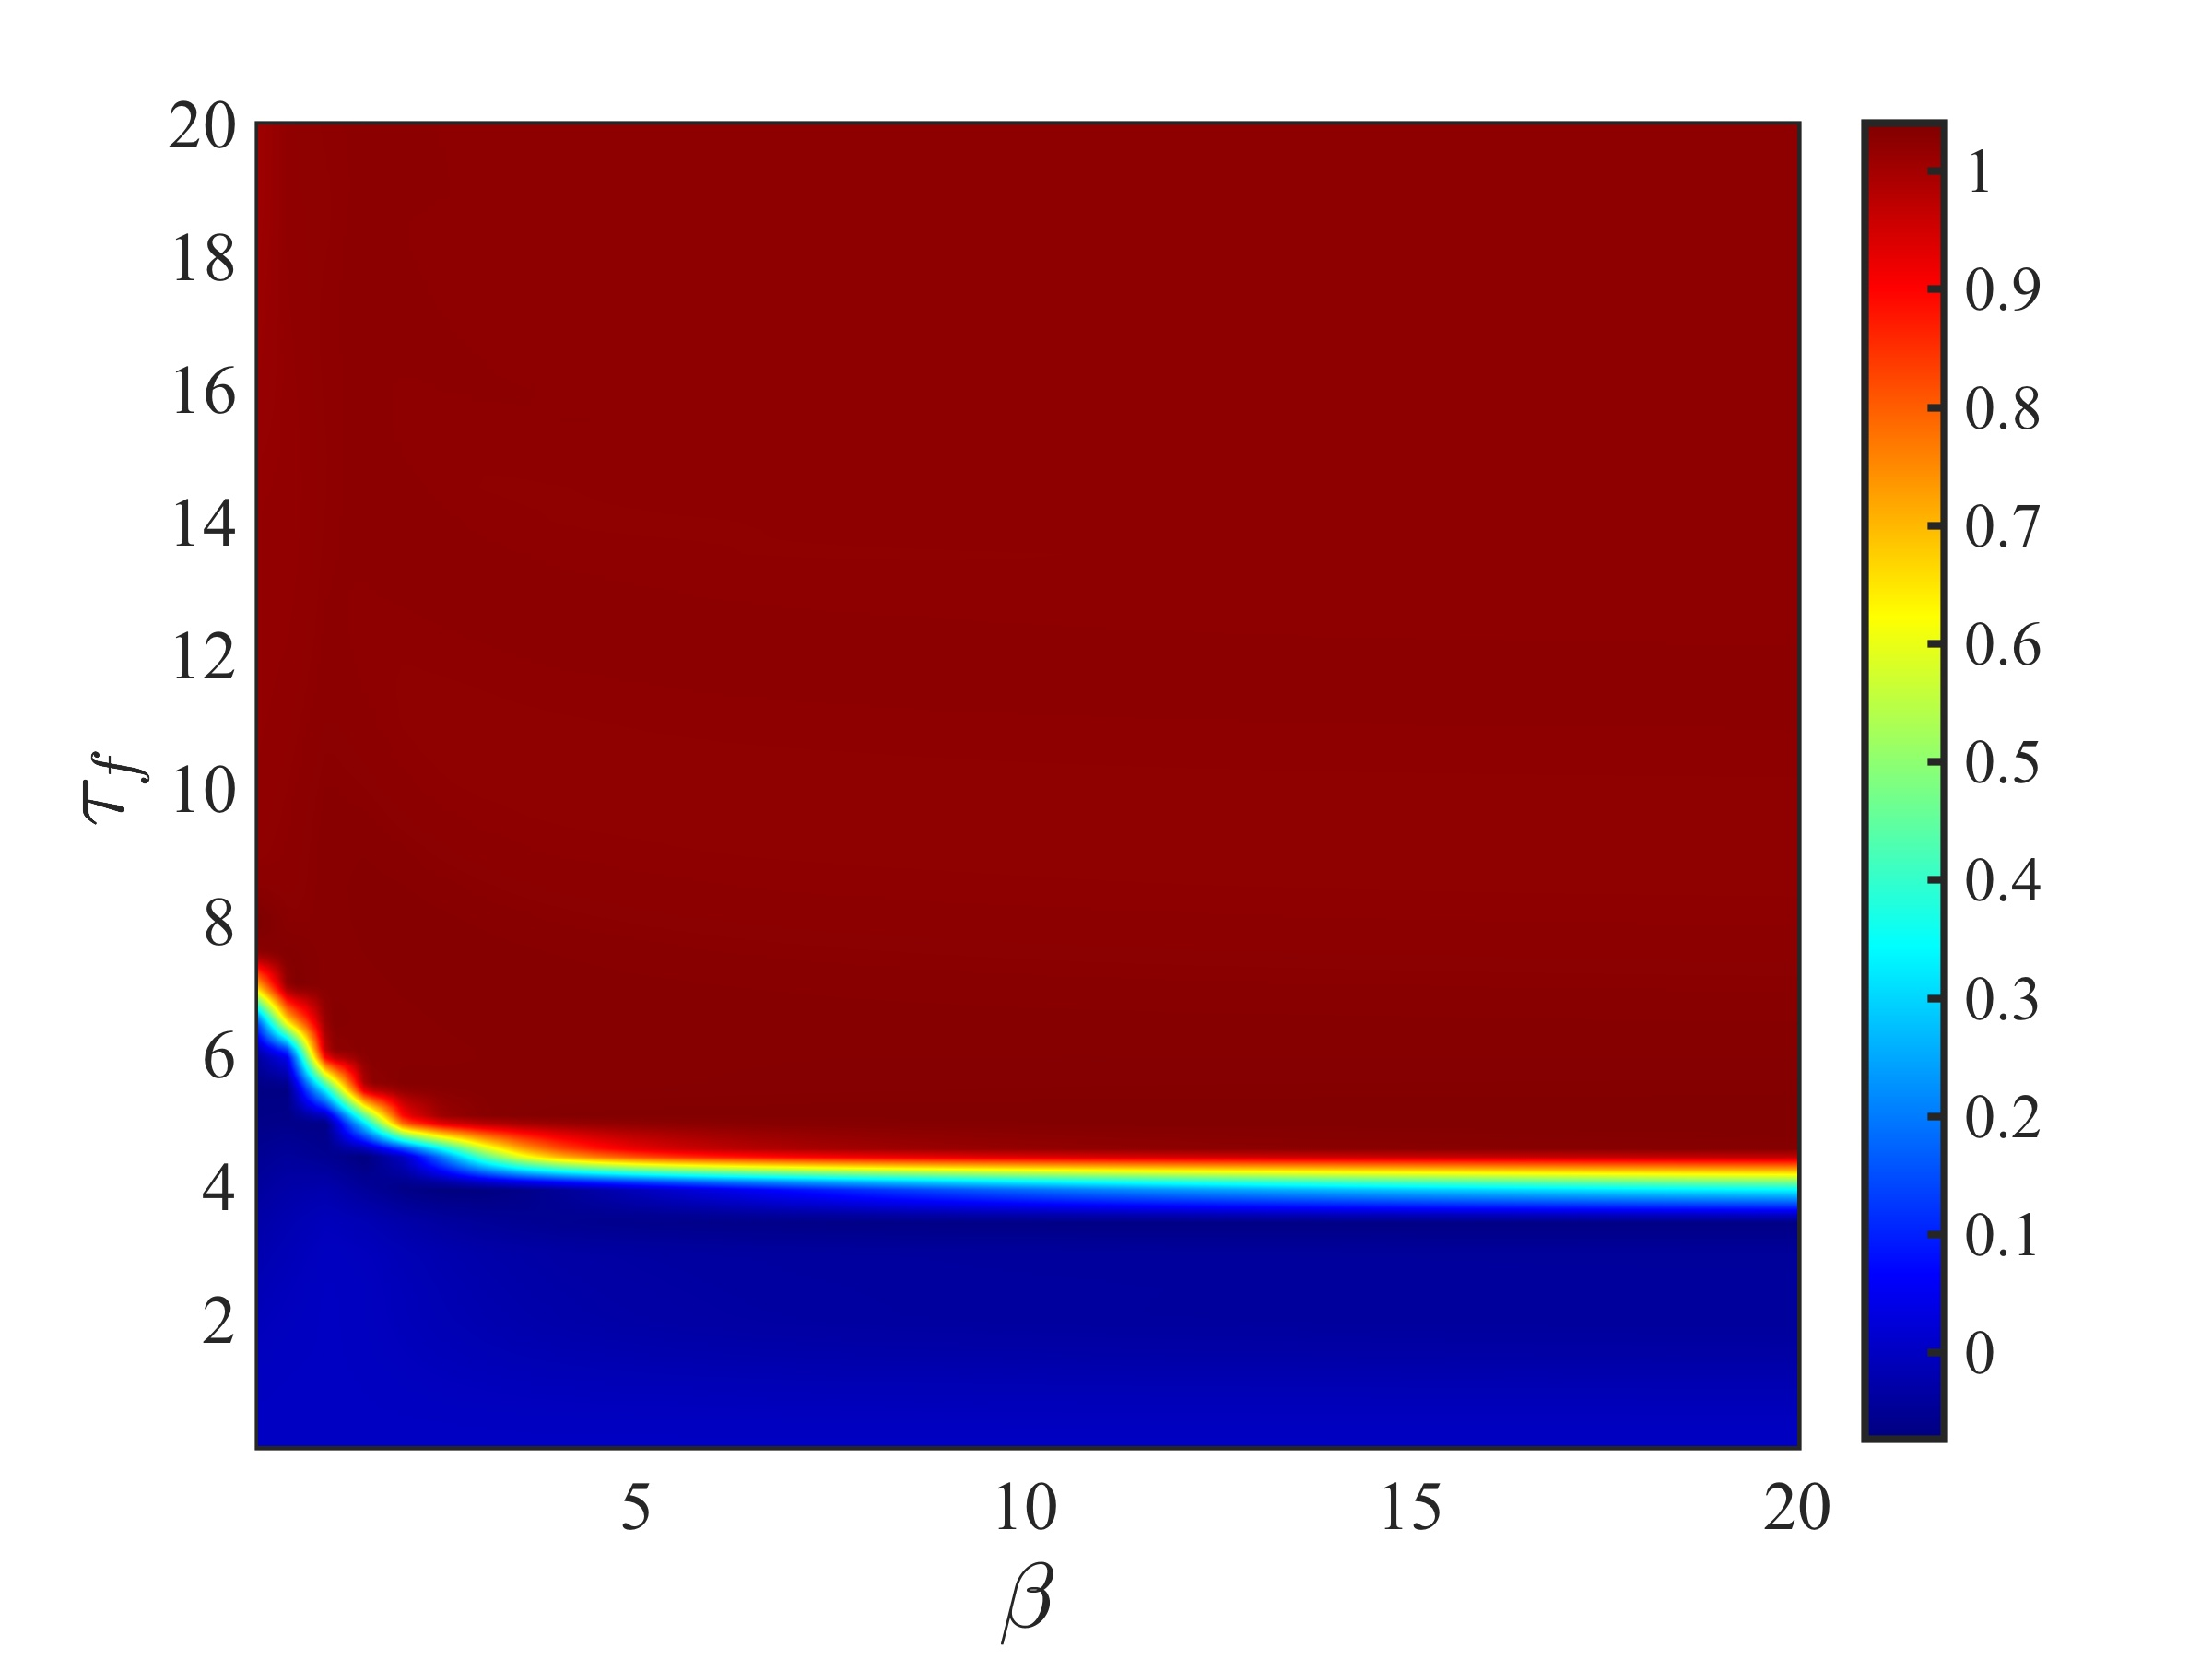
\includegraphics[width=\linewidth]{ACFatQIn.jpg}
\caption{} 
\end{subfigure}
%\hspace*{\fill}
\hspace*{-0.5cm}
\begin{subfigure}{0.5\textwidth}
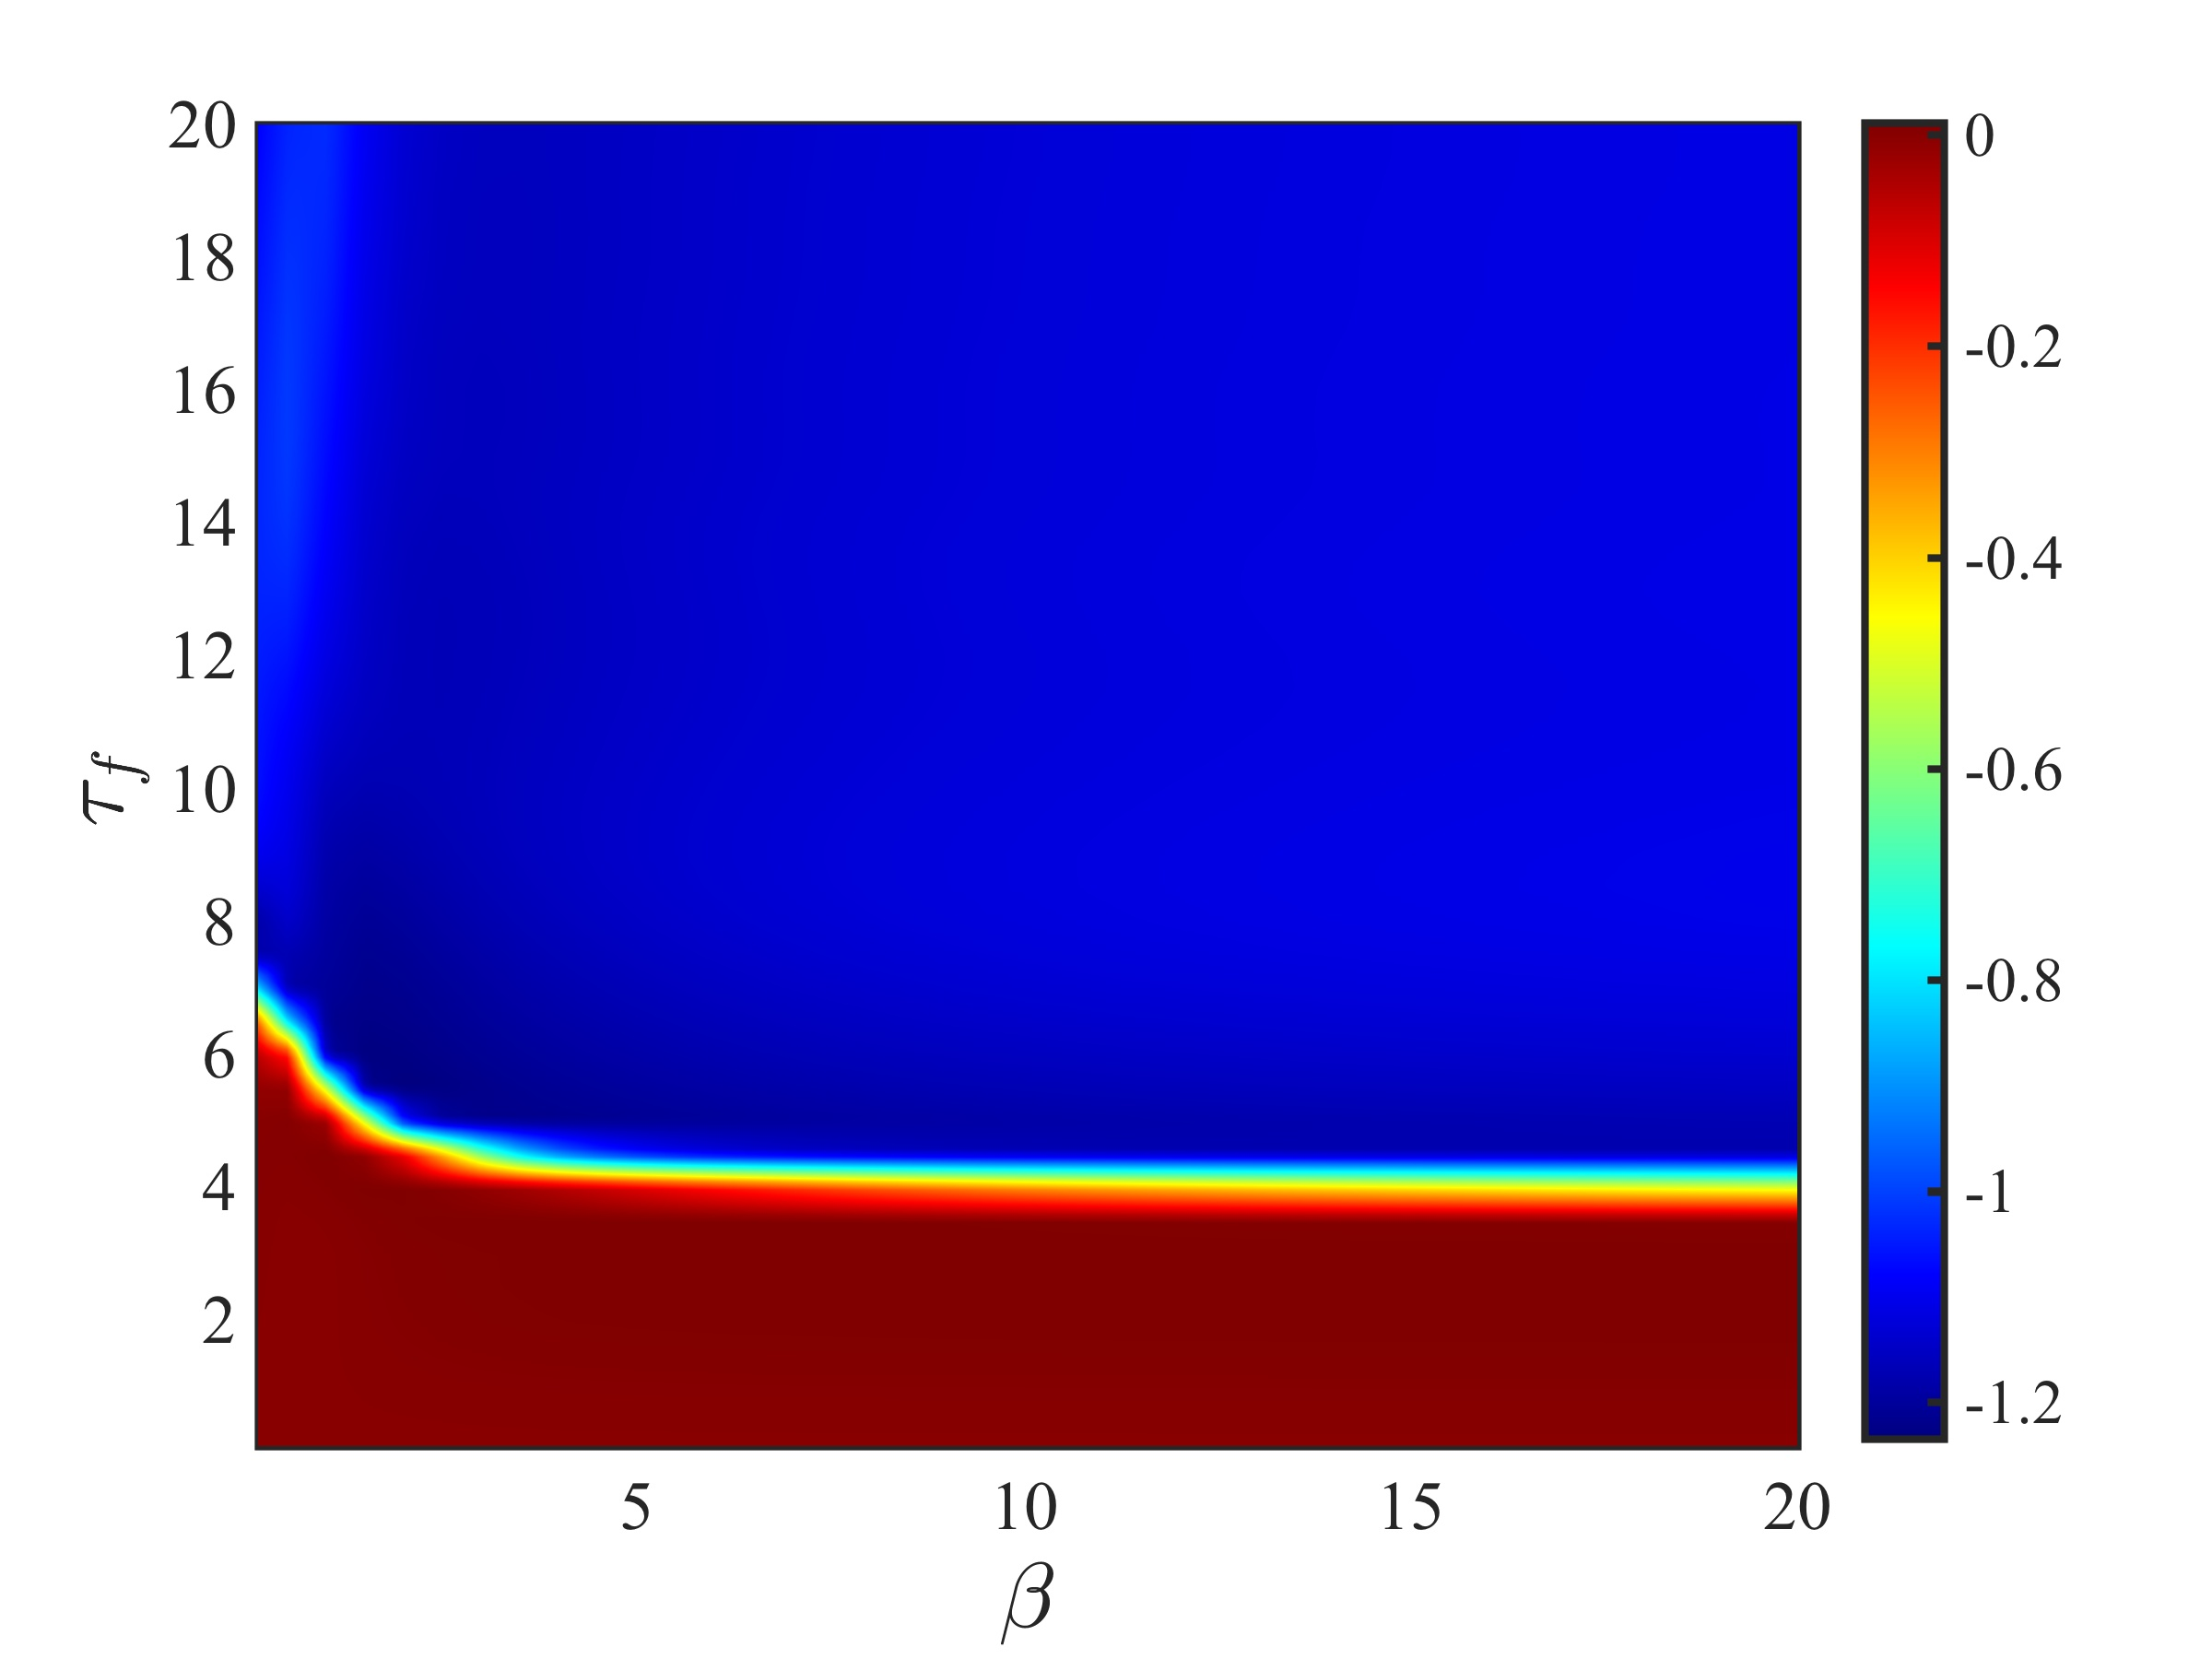
\includegraphics[width=\linewidth]{ACFatQOut.jpg} 
\caption{} 
\end{subfigure} 
\centerline{
%\hspace{1cm}
\begin{subfigure}{\textwidth}
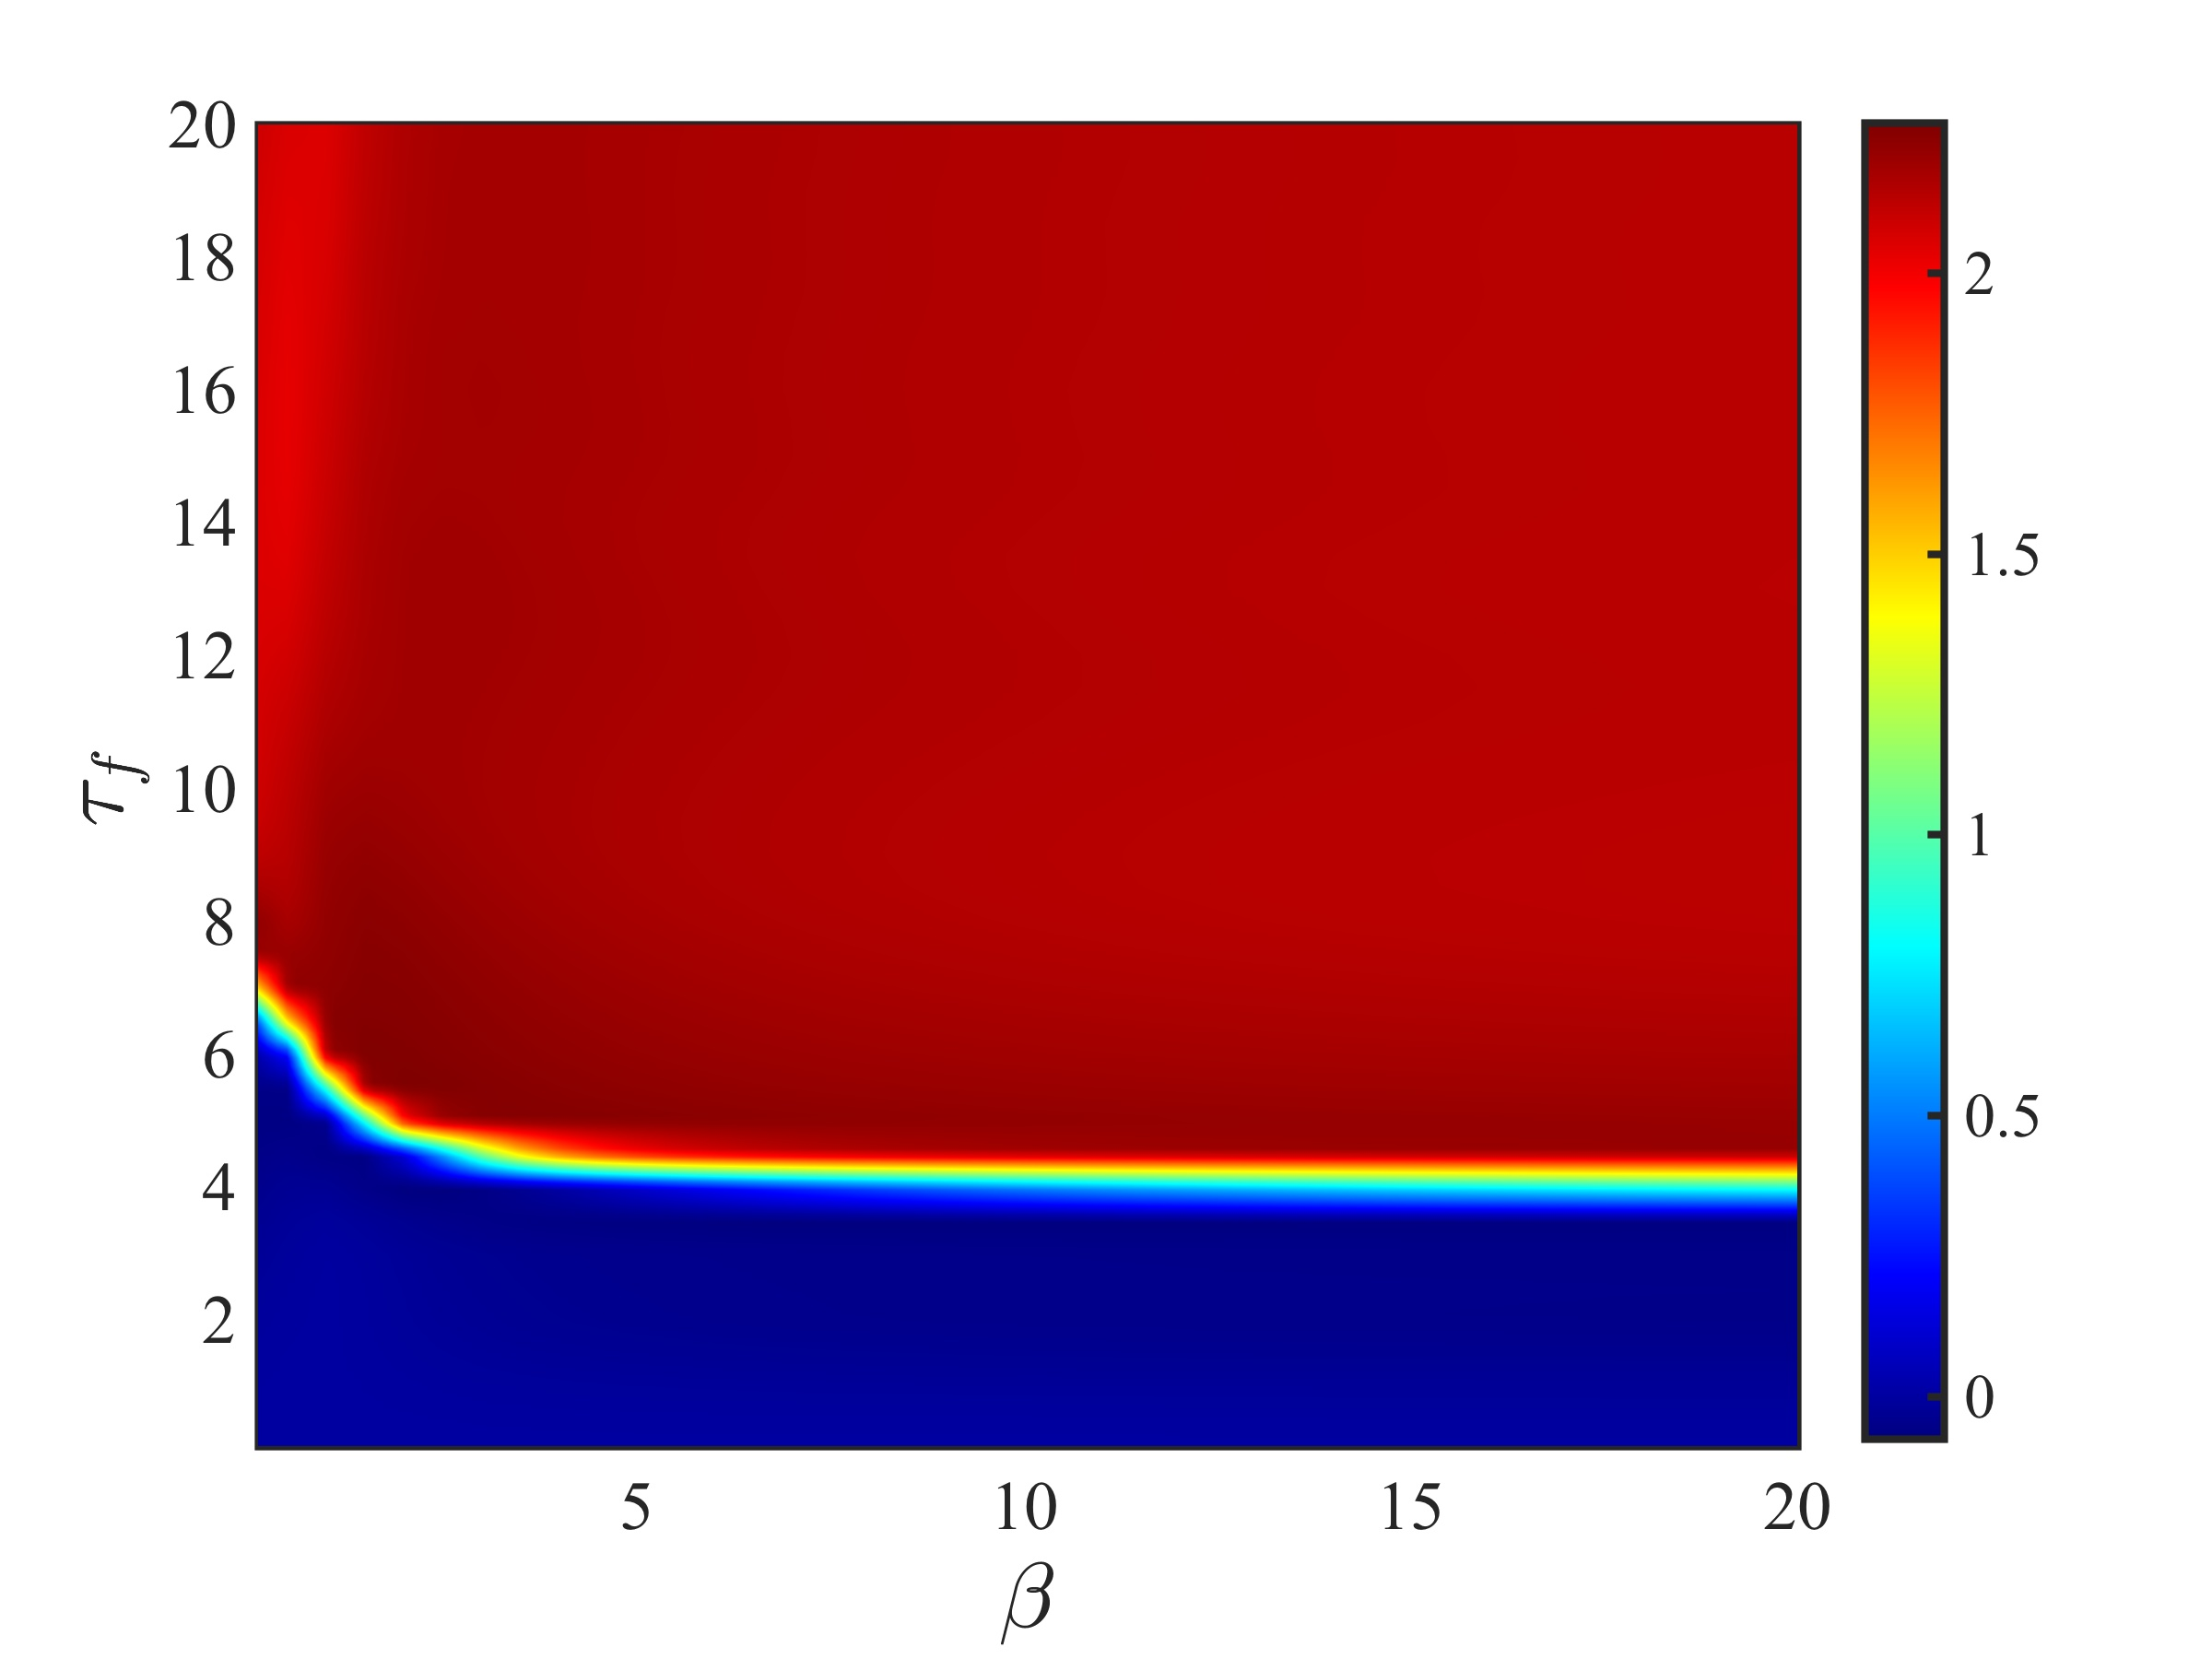
\includegraphics[width=\linewidth]{ACFatQDiff.jpg} 
\caption{} 
\end{subfigure} }
  \rule{35em}{0.5pt}
\caption[Power Ratios Inside and Outside Tweezer with $\sigma_\phi = 2$ and $h_\phi = 2$]{Power ratios as in Fig.~\ref{fig:ACSkinnyQ} but for a  tweezer with width $\sigma_\phi = 2$ and height $h_\phi = 2$.  The detuning for the system is $\Delta =  3.3830$.   Same layout as in Fig.~\ref{fig:ACSkinnyQ}.  The difference power ratio (c) defines the thresholds for tweezed CSs for all blue regions, no-CSs for all green regions, and non-tweezed CSs for all red regions.  
}
\label{fig:ACFatQ}
\end{figure}